% Options for packages loaded elsewhere
\PassOptionsToPackage{unicode}{hyperref}
\PassOptionsToPackage{hyphens}{url}
\PassOptionsToPackage{dvipsnames,svgnames,x11names}{xcolor}
%
\documentclass[
  letterpaper,
  DIV=11,
  numbers=noendperiod]{scrreprt}

\usepackage{amsmath,amssymb}
\usepackage{iftex}
\ifPDFTeX
  \usepackage[T1]{fontenc}
  \usepackage[utf8]{inputenc}
  \usepackage{textcomp} % provide euro and other symbols
\else % if luatex or xetex
  \usepackage{unicode-math}
  \defaultfontfeatures{Scale=MatchLowercase}
  \defaultfontfeatures[\rmfamily]{Ligatures=TeX,Scale=1}
\fi
\usepackage{lmodern}
\ifPDFTeX\else  
    % xetex/luatex font selection
\fi
% Use upquote if available, for straight quotes in verbatim environments
\IfFileExists{upquote.sty}{\usepackage{upquote}}{}
\IfFileExists{microtype.sty}{% use microtype if available
  \usepackage[]{microtype}
  \UseMicrotypeSet[protrusion]{basicmath} % disable protrusion for tt fonts
}{}
\makeatletter
\@ifundefined{KOMAClassName}{% if non-KOMA class
  \IfFileExists{parskip.sty}{%
    \usepackage{parskip}
  }{% else
    \setlength{\parindent}{0pt}
    \setlength{\parskip}{6pt plus 2pt minus 1pt}}
}{% if KOMA class
  \KOMAoptions{parskip=half}}
\makeatother
\usepackage{xcolor}
\setlength{\emergencystretch}{3em} % prevent overfull lines
\setcounter{secnumdepth}{5}
% Make \paragraph and \subparagraph free-standing
\makeatletter
\ifx\paragraph\undefined\else
  \let\oldparagraph\paragraph
  \renewcommand{\paragraph}{
    \@ifstar
      \xxxParagraphStar
      \xxxParagraphNoStar
  }
  \newcommand{\xxxParagraphStar}[1]{\oldparagraph*{#1}\mbox{}}
  \newcommand{\xxxParagraphNoStar}[1]{\oldparagraph{#1}\mbox{}}
\fi
\ifx\subparagraph\undefined\else
  \let\oldsubparagraph\subparagraph
  \renewcommand{\subparagraph}{
    \@ifstar
      \xxxSubParagraphStar
      \xxxSubParagraphNoStar
  }
  \newcommand{\xxxSubParagraphStar}[1]{\oldsubparagraph*{#1}\mbox{}}
  \newcommand{\xxxSubParagraphNoStar}[1]{\oldsubparagraph{#1}\mbox{}}
\fi
\makeatother

\usepackage{color}
\usepackage{fancyvrb}
\newcommand{\VerbBar}{|}
\newcommand{\VERB}{\Verb[commandchars=\\\{\}]}
\DefineVerbatimEnvironment{Highlighting}{Verbatim}{commandchars=\\\{\}}
% Add ',fontsize=\small' for more characters per line
\usepackage{framed}
\definecolor{shadecolor}{RGB}{241,243,245}
\newenvironment{Shaded}{\begin{snugshade}}{\end{snugshade}}
\newcommand{\AlertTok}[1]{\textcolor[rgb]{0.68,0.00,0.00}{#1}}
\newcommand{\AnnotationTok}[1]{\textcolor[rgb]{0.37,0.37,0.37}{#1}}
\newcommand{\AttributeTok}[1]{\textcolor[rgb]{0.40,0.45,0.13}{#1}}
\newcommand{\BaseNTok}[1]{\textcolor[rgb]{0.68,0.00,0.00}{#1}}
\newcommand{\BuiltInTok}[1]{\textcolor[rgb]{0.00,0.23,0.31}{#1}}
\newcommand{\CharTok}[1]{\textcolor[rgb]{0.13,0.47,0.30}{#1}}
\newcommand{\CommentTok}[1]{\textcolor[rgb]{0.37,0.37,0.37}{#1}}
\newcommand{\CommentVarTok}[1]{\textcolor[rgb]{0.37,0.37,0.37}{\textit{#1}}}
\newcommand{\ConstantTok}[1]{\textcolor[rgb]{0.56,0.35,0.01}{#1}}
\newcommand{\ControlFlowTok}[1]{\textcolor[rgb]{0.00,0.23,0.31}{\textbf{#1}}}
\newcommand{\DataTypeTok}[1]{\textcolor[rgb]{0.68,0.00,0.00}{#1}}
\newcommand{\DecValTok}[1]{\textcolor[rgb]{0.68,0.00,0.00}{#1}}
\newcommand{\DocumentationTok}[1]{\textcolor[rgb]{0.37,0.37,0.37}{\textit{#1}}}
\newcommand{\ErrorTok}[1]{\textcolor[rgb]{0.68,0.00,0.00}{#1}}
\newcommand{\ExtensionTok}[1]{\textcolor[rgb]{0.00,0.23,0.31}{#1}}
\newcommand{\FloatTok}[1]{\textcolor[rgb]{0.68,0.00,0.00}{#1}}
\newcommand{\FunctionTok}[1]{\textcolor[rgb]{0.28,0.35,0.67}{#1}}
\newcommand{\ImportTok}[1]{\textcolor[rgb]{0.00,0.46,0.62}{#1}}
\newcommand{\InformationTok}[1]{\textcolor[rgb]{0.37,0.37,0.37}{#1}}
\newcommand{\KeywordTok}[1]{\textcolor[rgb]{0.00,0.23,0.31}{\textbf{#1}}}
\newcommand{\NormalTok}[1]{\textcolor[rgb]{0.00,0.23,0.31}{#1}}
\newcommand{\OperatorTok}[1]{\textcolor[rgb]{0.37,0.37,0.37}{#1}}
\newcommand{\OtherTok}[1]{\textcolor[rgb]{0.00,0.23,0.31}{#1}}
\newcommand{\PreprocessorTok}[1]{\textcolor[rgb]{0.68,0.00,0.00}{#1}}
\newcommand{\RegionMarkerTok}[1]{\textcolor[rgb]{0.00,0.23,0.31}{#1}}
\newcommand{\SpecialCharTok}[1]{\textcolor[rgb]{0.37,0.37,0.37}{#1}}
\newcommand{\SpecialStringTok}[1]{\textcolor[rgb]{0.13,0.47,0.30}{#1}}
\newcommand{\StringTok}[1]{\textcolor[rgb]{0.13,0.47,0.30}{#1}}
\newcommand{\VariableTok}[1]{\textcolor[rgb]{0.07,0.07,0.07}{#1}}
\newcommand{\VerbatimStringTok}[1]{\textcolor[rgb]{0.13,0.47,0.30}{#1}}
\newcommand{\WarningTok}[1]{\textcolor[rgb]{0.37,0.37,0.37}{\textit{#1}}}

\providecommand{\tightlist}{%
  \setlength{\itemsep}{0pt}\setlength{\parskip}{0pt}}\usepackage{longtable,booktabs,array}
\usepackage{calc} % for calculating minipage widths
% Correct order of tables after \paragraph or \subparagraph
\usepackage{etoolbox}
\makeatletter
\patchcmd\longtable{\par}{\if@noskipsec\mbox{}\fi\par}{}{}
\makeatother
% Allow footnotes in longtable head/foot
\IfFileExists{footnotehyper.sty}{\usepackage{footnotehyper}}{\usepackage{footnote}}
\makesavenoteenv{longtable}
\usepackage{graphicx}
\makeatletter
\def\maxwidth{\ifdim\Gin@nat@width>\linewidth\linewidth\else\Gin@nat@width\fi}
\def\maxheight{\ifdim\Gin@nat@height>\textheight\textheight\else\Gin@nat@height\fi}
\makeatother
% Scale images if necessary, so that they will not overflow the page
% margins by default, and it is still possible to overwrite the defaults
% using explicit options in \includegraphics[width, height, ...]{}
\setkeys{Gin}{width=\maxwidth,height=\maxheight,keepaspectratio}
% Set default figure placement to htbp
\makeatletter
\def\fps@figure{htbp}
\makeatother
% definitions for citeproc citations
\NewDocumentCommand\citeproctext{}{}
\NewDocumentCommand\citeproc{mm}{%
  \begingroup\def\citeproctext{#2}\cite{#1}\endgroup}
\makeatletter
 % allow citations to break across lines
 \let\@cite@ofmt\@firstofone
 % avoid brackets around text for \cite:
 \def\@biblabel#1{}
 \def\@cite#1#2{{#1\if@tempswa , #2\fi}}
\makeatother
\newlength{\cslhangindent}
\setlength{\cslhangindent}{1.5em}
\newlength{\csllabelwidth}
\setlength{\csllabelwidth}{3em}
\newenvironment{CSLReferences}[2] % #1 hanging-indent, #2 entry-spacing
 {\begin{list}{}{%
  \setlength{\itemindent}{0pt}
  \setlength{\leftmargin}{0pt}
  \setlength{\parsep}{0pt}
  % turn on hanging indent if param 1 is 1
  \ifodd #1
   \setlength{\leftmargin}{\cslhangindent}
   \setlength{\itemindent}{-1\cslhangindent}
  \fi
  % set entry spacing
  \setlength{\itemsep}{#2\baselineskip}}}
 {\end{list}}
\usepackage{calc}
\newcommand{\CSLBlock}[1]{\hfill\break\parbox[t]{\linewidth}{\strut\ignorespaces#1\strut}}
\newcommand{\CSLLeftMargin}[1]{\parbox[t]{\csllabelwidth}{\strut#1\strut}}
\newcommand{\CSLRightInline}[1]{\parbox[t]{\linewidth - \csllabelwidth}{\strut#1\strut}}
\newcommand{\CSLIndent}[1]{\hspace{\cslhangindent}#1}

\KOMAoption{captions}{tableheading}
\makeatletter
\@ifpackageloaded{bookmark}{}{\usepackage{bookmark}}
\makeatother
\makeatletter
\@ifpackageloaded{caption}{}{\usepackage{caption}}
\AtBeginDocument{%
\ifdefined\contentsname
  \renewcommand*\contentsname{Table of contents}
\else
  \newcommand\contentsname{Table of contents}
\fi
\ifdefined\listfigurename
  \renewcommand*\listfigurename{List of Figures}
\else
  \newcommand\listfigurename{List of Figures}
\fi
\ifdefined\listtablename
  \renewcommand*\listtablename{List of Tables}
\else
  \newcommand\listtablename{List of Tables}
\fi
\ifdefined\figurename
  \renewcommand*\figurename{Figure}
\else
  \newcommand\figurename{Figure}
\fi
\ifdefined\tablename
  \renewcommand*\tablename{Table}
\else
  \newcommand\tablename{Table}
\fi
}
\@ifpackageloaded{float}{}{\usepackage{float}}
\floatstyle{ruled}
\@ifundefined{c@chapter}{\newfloat{codelisting}{h}{lop}}{\newfloat{codelisting}{h}{lop}[chapter]}
\floatname{codelisting}{Listing}
\newcommand*\listoflistings{\listof{codelisting}{List of Listings}}
\makeatother
\makeatletter
\makeatother
\makeatletter
\@ifpackageloaded{caption}{}{\usepackage{caption}}
\@ifpackageloaded{subcaption}{}{\usepackage{subcaption}}
\makeatother

\ifLuaTeX
  \usepackage{selnolig}  % disable illegal ligatures
\fi
\usepackage{bookmark}

\IfFileExists{xurl.sty}{\usepackage{xurl}}{} % add URL line breaks if available
\urlstyle{same} % disable monospaced font for URLs
\hypersetup{
  pdftitle={Introduction to Stochastic Processes},
  pdfauthor={Thiyanga S. Talagala},
  colorlinks=true,
  linkcolor={blue},
  filecolor={Maroon},
  citecolor={Blue},
  urlcolor={Blue},
  pdfcreator={LaTeX via pandoc}}


\title{Introduction to Stochastic Processes}
\author{Thiyanga S. Talagala}
\date{}

\begin{document}
\maketitle

\renewcommand*\contentsname{Table of contents}
{
\hypersetup{linkcolor=}
\setcounter{tocdepth}{2}
\tableofcontents
}

\bookmarksetup{startatroot}

\chapter*{Preface}\label{preface}
\addcontentsline{toc}{chapter}{Preface}

\markboth{Preface}{Preface}

This is a Quarto book.

To learn more about Quarto books visit
\url{https://quarto.org/docs/books}.

\bookmarksetup{startatroot}

\chapter{Introduction}\label{introduction}

\section{What is a Stochastic
Process?}\label{what-is-a-stochastic-process}

First, let's see what does ``stochastic'' mean? The meaning of
``stochastic'' is \textbf{random}. The term ``process'' refers to a
mathematical or statistical model that describes the evolution of a
random variable over time. In the study of a stochastic process, we
examine a collection of random variables indexed by a certain parameter,
typically time, representing the evolution of a system over a series of
discrete or continuous instances.

For example, suppose we monitor the weather condition every hour in a
day sunny, rainy, and cloudy. Then you are essentially observing a
stochastic process. This process describes how the weather condition
evolves over time.

Can we describe this situation using a single random variable? No, we
cannot. We need a sequence of random variables index by time as follows:

\(X_0\) - weather condition from 00:00 to 01:00

\(X_1\) - weather condition from 01:00 to 02:00

.

.

.

\(X_{23}\) - weather condition from 23:00 - 00:00

The above scenario can be framed as a stochastic process. Here's how it
relates to the concept of a stochastic process:

\textbf{Time index:} The time index is the hour of the day as 0, 1, 2,
3, \ldots{} 23. Each hour is a specific point in time.

\textbf{Random variable:} The weather conditions at each hour can be
viewed as random variables. These random variables can be take different
values such as sunny, rainy and cloudy. The weather conditions
sunny,rainy and cloudy are called \emph{states} (see Section for more
information).

In many real life situations, observations are made over a period of
time. Stochastic processes are used to model and analyze such
time-dependent random phenomena, allowing you to study the probabilistic
behavior and make predictions about future states based on past
observations. When dealing with stochastic processes, we can address
various probabilistic questions, including but not limited to:

\begin{enumerate}
\def\labelenumi{\arabic{enumi}.}
\item
  \textbf{Conditional probabilities: }For instance, given that the
  weather has been cloudy for the first five hours of the day, you can
  use the stochastic process to estimate the likelihood of it remaining
  cloudy or changing to a different condition in the next hour.
\item
  \textbf{Time to an event: } For example, you can estimate how long it
  will take for the weather to change from cloudy to sunny.
\item
  \textbf{Transition probabilities: } For instance, you can determine
  the likelihood of going from a rainy day to a sunny day or vice versa.
\item
  \textbf{Frequency of Events:} You can examine the frequency of
  specific events occurring within a given time frame.
\end{enumerate}

These are just a few examples of the probabilistic questions that can be
addressed using stochastic processes. The specific questions you can
answer will depend on the nature of the process and the data available
for analysis.

\section{Definition of a stochastic
process}\label{definition-of-a-stochastic-process}

\textbf{Definition 1}

A stochastic process is a collection of random variables
\(\{X_t, t\in T\}\) or \({X(t), t \in T}\) where \(T\) is an index
set.That is for each \(t \in T\), the random variable \(X_t\) (or
\(X(t)\)) is a random variable.

\section{Parameter space}\label{parameter-space}

In definition 1, the index set \(T\) is called the parameter space. It
is usually interpreted as a time variable, telling us when the process
is measured. The parameter space can be discrete or continuous.

\subsection{Discrete-parameter
process}\label{discrete-parameter-process}

When \(T\) is a countable set, the process is said to be a
discrete-parameter process. A discrete-parameter stochastic process is
defined as follows:

\[\{X_t: t \in T\}\] \textbf{Example:} Number of Customers arriving each
hour to a particular super market (Discrete Parameter Space)

In this scenario, you are interested in the number of customers arriving
during each discrete time interval, typically on an hourly basis.

\subsection{Continuous-parameter
space}\label{continuous-parameter-space}

When \(T\) is an interval of the real line, the process is said to be a
continuous-parameter process. A continuous-parameter stochastic process
is defined as follows:

\[\{X(t): t \in T\}\]

\textbf{Example 1:} Number of Customers Arriving from 8 AM to 10 PM
(Continuous Parameter Space):

In this scenario, you are interested in the total number of customers
arriving over a continuous time period, specifically from 8 AM to 10 PM.

\section{State space}\label{state-space}

The set of possible values of an individual random variable \(X_t\) or
\(X(t)\) of a stochastic process is called the state space. The state
space can be discrete or continuous.

\section{Random Variable in Probability Theory vs Stochastic
Theory}\label{random-variable-in-probability-theory-vs-stochastic-theory}

\subsection{Probability theory}\label{probability-theory}

Let \((\Omega, \mathscr{F}, \mathbb{P})\) be a probability space. A
measurable mapping \(X: \Omega \rightarrow \mathbb{R}\) is called a
random variable. The \(X(\omega)\) for \(\omega \in \Omega\) iscalled a
realization of \(X\).

\textbf{Example:}

\subsection{Stochastic theory}\label{stochastic-theory}

Suppose that \((\Omega, \mathscr{F}, \mathbb{P})\) is a probability
space, the function \(X: T \times \Omega \rightarrow \mathbb{R}\) .

\begin{itemize}
\tightlist
\item
  We will always assume that the cardinality of \(T\) is infinite,
  either countable or uncountable.
\end{itemize}

If \(T=\mathbb{Z}^+\) then we called \(X\) a discrete time stochastic
process.

If \(I = [0,\infty)\), then \(X\) is said to be a continuous time
stochastic processes.

\section{Sample path (trajectory) of a stochastic
process}\label{sample-path-trajectory-of-a-stochastic-process}

The function \(t \rightarrow X_t(\omega)\)
(\(t \rightarrow X(t)(\omega)\)) is called a sample path of the
stochastic process. For each

\textbf{Example:}

\section{Types of Stochastic
Processes}\label{types-of-stochastic-processes}

Depending on the parameter space and state space we can define four type
of stochastic processes.

\textbf{1. Discrete-Parameter Discrete-State Space Stochastic
Processes:}

\begin{itemize}
\item
  Parameter Space: Discrete
\item
  State Space: Discrete
\item
  Examples: Assessment of crop condition during routine field
  inspections in agriculture is categorized as: healthy, pest-infested,
  diseased, damaged. These field inspections are typically conducted at
  regular intervals, such as once a week
\end{itemize}

\textbf{2. Continuous-Parameter Discrete-State Space Stochastic
Processes:}

\begin{itemize}
\item
  Parameter Space: Continuous
\item
  State Space: Discrete
\item
  Examples:
\end{itemize}

\textbf{3. Discrete-Parameter Continous-State Space Stochastic
Processes:}

\begin{itemize}
\item
  Parameter Space: Discrete
\item
  State Space: Continuous
\item
  Examples:
\end{itemize}

\textbf{4. Continuous-Parameter Continuous-State Space Stochastic
Processes:}

\begin{itemize}
\item
  Parameter Space: Continuous
\item
  State Space: Continuous
\item
  Examples:
\end{itemize}

\section{Stochastic proceses vs Time
series}\label{stochastic-proceses-vs-time-series}

Figure Figure~\ref{fig-plot1} shows a weekly dengue cases in Sri Lanka
from 2006 - Week 52 to 2023 - Week 8. The data are available in the
denguedatahub package in R (\textbf{dengudatahub?}). The first few rows
of the dataset is shown below.

\begin{longtable}[]{@{}rrlllr@{}}
\toprule\noalign{}
year & week & start.date & end.date & district & cases \\
\midrule\noalign{}
\endhead
\bottomrule\noalign{}
\endlastfoot
2006 & 52 & 2006-12-23 & 2006-12-29 & Colombo & 71 \\
2007 & 1 & 2006-12-30 & 2007-01-05 & Colombo & 40 \\
2007 & 2 & 2007-01-06 & 2007-01-12 & Colombo & 43 \\
2007 & 3 & 2007-01-13 & 2007-01-19 & Colombo & 38 \\
2007 & 4 & 2007-01-20 & 2007-01-26 & Colombo & 52 \\
2007 & 5 & 2007-01-27 & 2007-02-02 & Colombo & 69 \\
\end{longtable}

Let's define the set of random variables as follows:

\(X_0\) - Cases of dengue during the fifty second week of 2006

\(X_1\) - Cases of dengue during the first week of 2007

\(X_2\) - Cases of dengue during the second week of 2007

.

.

.

Do you consider Figure~\ref{fig-plot1} as a visual representation of the
above \textbf{Stochastic Process}?

\begin{Shaded}
\begin{Highlighting}[]
\FunctionTok{library}\NormalTok{(denguedatahub) }\CommentTok{\# to load data}
\FunctionTok{library}\NormalTok{(ggplot2) }\CommentTok{\# for plotting}
\FunctionTok{data}\NormalTok{(srilanka\_weekly\_data)}
\NormalTok{srilanka\_weekly\_data }\SpecialCharTok{|\textgreater{}} 
\NormalTok{  dplyr}\SpecialCharTok{::}\FunctionTok{filter}\NormalTok{(district }\SpecialCharTok{==} \StringTok{"Colombo"}\NormalTok{) }\SpecialCharTok{|\textgreater{}}
\NormalTok{ggplot2}\SpecialCharTok{::}\FunctionTok{ggplot}\NormalTok{(}\FunctionTok{aes}\NormalTok{(}\AttributeTok{x=}\NormalTok{start.date, }\AttributeTok{y=}\NormalTok{cases)) }\SpecialCharTok{+} 
  \FunctionTok{geom\_line}\NormalTok{()  }\SpecialCharTok{+} 
  \FunctionTok{scale\_x\_date}\NormalTok{(}\AttributeTok{date\_breaks =} \StringTok{"1 year"}\NormalTok{, }\AttributeTok{date\_labels =} \StringTok{"\%Y"}\NormalTok{) }\SpecialCharTok{+} 
  \FunctionTok{theme}\NormalTok{(}\AttributeTok{axis.text.x =} \FunctionTok{element\_text}\NormalTok{(}\AttributeTok{angle =} \DecValTok{90}\NormalTok{, }\AttributeTok{vjust =} \FloatTok{0.5}\NormalTok{, }\AttributeTok{hjust=}\DecValTok{1}\NormalTok{)) }\SpecialCharTok{+} \FunctionTok{xlab}\NormalTok{(}\StringTok{"Time"}\NormalTok{)}
\end{Highlighting}
\end{Shaded}

\begin{figure}[H]

\centering{

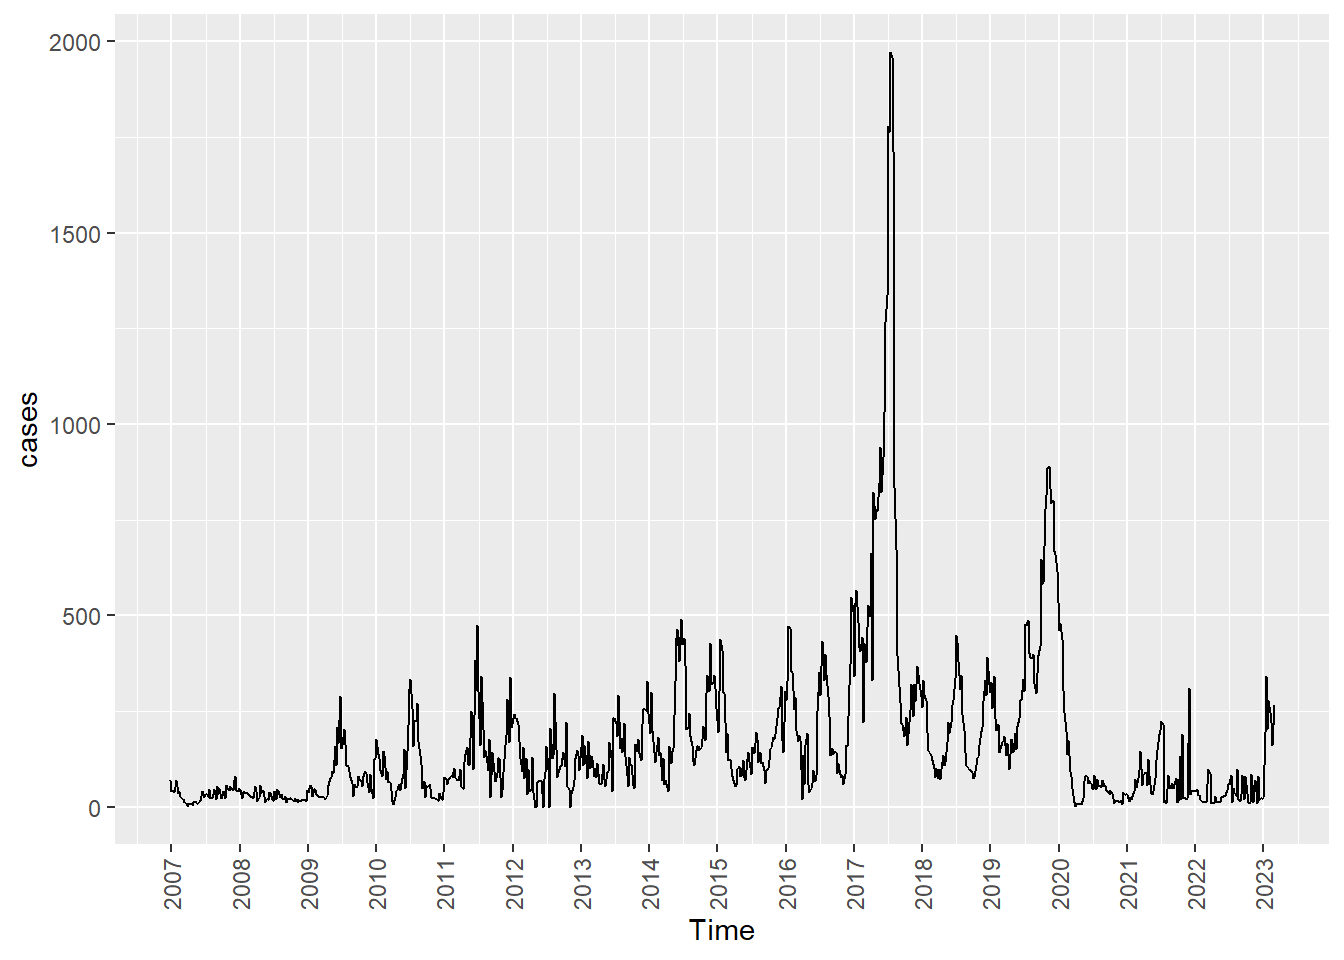
\includegraphics{intro_files/figure-pdf/fig-plot1-1.pdf}

}

\caption{\label{fig-plot1}Weekly dengue cases in Sri Lanka from 2007 to
2023 August}

\end{figure}%

The answer is ``No''. Figure~\ref{fig-plot1} is not a visual
representation of the stochastic process. It is a realization of the
above stochastic process. According to the data set in the fifty second
week of 2006, there were 76 cases were reported. This is the observed
value of the random variable \(X_0\). Similarly, the observed value of
the random variable \(X_1\) is 40. Hence, Figure~\ref{fig-plot1}
represents the set of observed values of the the stochastic process.
This is called a time series. ``In other words, time series is a
realization of a stochastic process. When we say a time series is a
realization, we mean that it represents a specific outcome or path or
trajectory of a stochastic process. A realization is essentially a
particular observed sequence of values that the process can take.
Therefore, when we say a time series is a realization of a stochastic
process, we are highlighting that the observed sequence of data points
in a time series is \textbf{one possible outcome} of a random process
that unfolds over time. The stochastic nature implies that, even though
the underlying process has certain statistical properties, the specific
values observed at any given point in time are not predetermined and can
exhibit variability.

\section{Stochastic process vs a deterministic
process}\label{stochastic-process-vs-a-deterministic-process}

Consider the following data generating process and its visual
representation. Let's define the set of random variables as follows:

\(X_0\) - value at time \(t=1\)

\(X_1\) - value at time \(t=2\)

\(X_2\) - value at time \(t=3\)

.

.

.

Do you consider Figure~\ref{fig-plot2} as a realization of a stochastic
process?

\begin{Shaded}
\begin{Highlighting}[]
\NormalTok{t }\OtherTok{\textless{}{-}} \DecValTok{1}\SpecialCharTok{:}\DecValTok{100}
\NormalTok{xt }\OtherTok{\textless{}{-}} \FunctionTok{sin}\NormalTok{(}\DecValTok{2}\SpecialCharTok{*}\NormalTok{pi}\SpecialCharTok{*}\NormalTok{t)}
\NormalTok{df }\OtherTok{\textless{}{-}} \FunctionTok{data.frame}\NormalTok{(}\AttributeTok{xt=}\NormalTok{xt, }\AttributeTok{t=}\NormalTok{t)}
\FunctionTok{ggplot}\NormalTok{(}\AttributeTok{data=}\NormalTok{df, }\FunctionTok{aes}\NormalTok{(}\AttributeTok{x=}\NormalTok{t, }\AttributeTok{y=}\NormalTok{xt)) }\SpecialCharTok{+} 
  \FunctionTok{geom\_point}\NormalTok{() }\SpecialCharTok{+} 
  \FunctionTok{geom\_line}\NormalTok{()}
\end{Highlighting}
\end{Shaded}

\begin{figure}[H]

\centering{

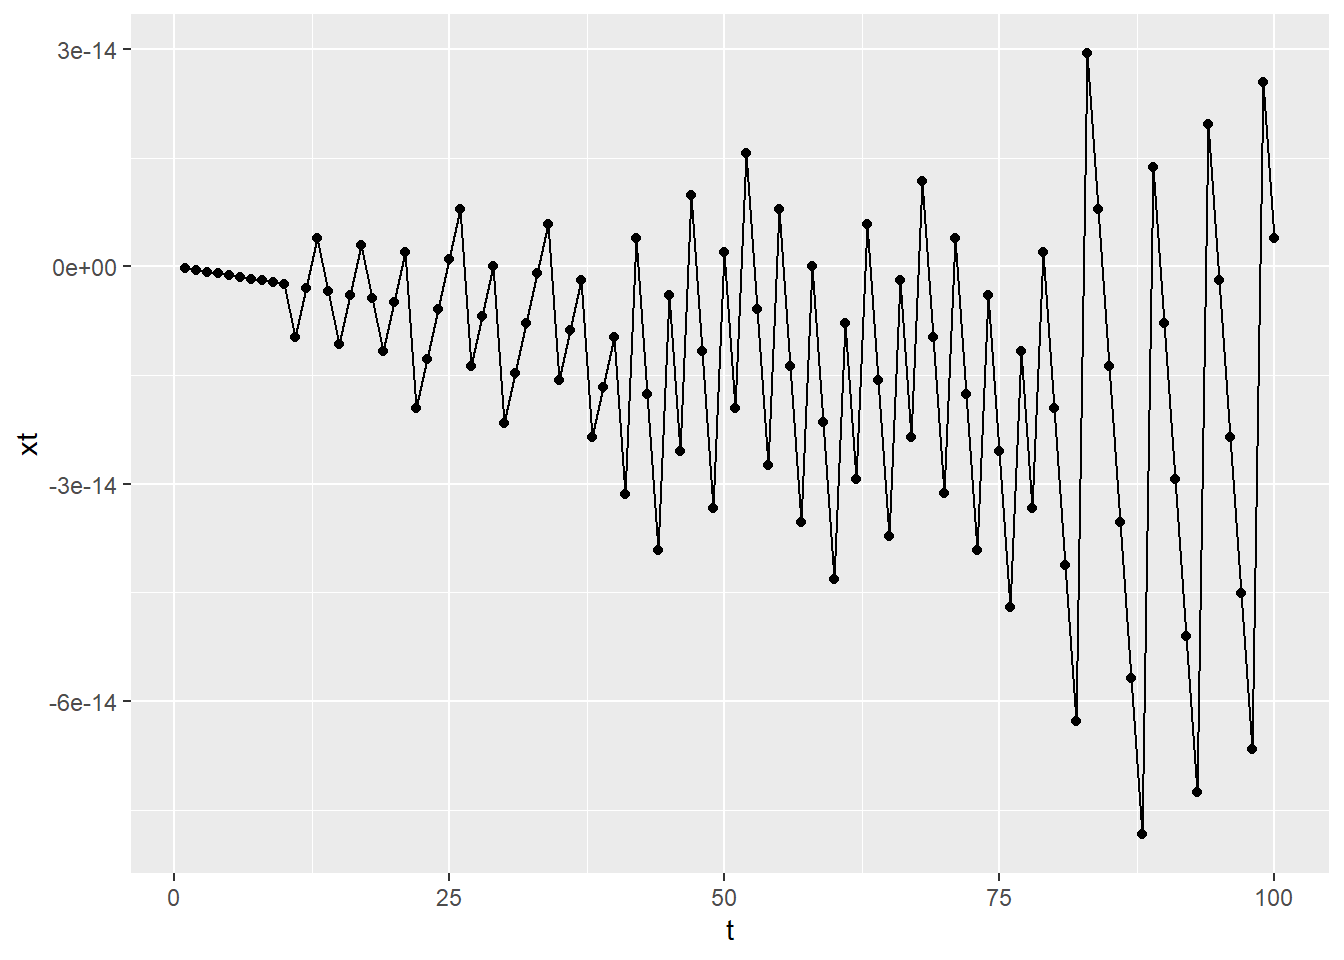
\includegraphics{intro_files/figure-pdf/fig-plot2-1.pdf}

}

\caption{\label{fig-plot2}Visual representation of data}

\end{figure}%

The answer is ``No''. The reason is when you observe the above R-code
you can see the values are generated based on the function
\(\sin(2 \pi t)\). Hence, there is no randomness associated with he
random variables. This type of process is called a deterministic
process.

\section{Stationary condition of a stochastic
process}\label{stationary-condition-of-a-stochastic-process}

\section{Independent increments condition of a stochastic
process}\label{independent-increments-condition-of-a-stochastic-process}

\section{Stationary increments condition of a stochastic
process}\label{stationary-increments-condition-of-a-stochastic-process}

\section{Stochastic processes vs probaility calculation in a single
random
variable}\label{stochastic-processes-vs-probaility-calculation-in-a-single-random-variable}

\section{Applications of stochastic
processes}\label{applications-of-stochastic-processes}

\bookmarksetup{startatroot}

\chapter{Discrete Parameter Markov
Chains}\label{discrete-parameter-markov-chains}

\section{Introduction}\label{introduction-1}

A discrete parameter Markov chain process is a modeling approach used to
represent systems that evolve over time in \textbf{discrete steps},
where the \textbf{future state depends only on the current state}. This
is very useful in analyzing distinct states and transitions. Discrete
Parameter Markov Chains is also known as ``Discrete-time Markov
Chains''.

\textbf{Definition}

Let \(\{X_n; n = 0, 1, 2, ...\}\) be a stochastic process that takes on
a finite or countable number of possible values. If \(X_n=i,\) then the
process is said to be in state \(i\) at time \(n\).

The discrete-parameter, discrete state stochastic process
\(\{X_n; n=0, 1, 2,...\}\) is called a \textbf{discrete-parameter Markov
chain} if for all states \(i_0, i_1,...i_{n-1}, i, j\) and all
\(n \geq 0\),

\[P(X_{n+1}=j|X_n=i, X_{n-1}=i_{n-1}, ..., X_1=i_1, X_0=i_0) = P(X_{n+1}=j|X_n=i).\]

This means, a stochastic process is a Markov chain if the probability of
moving to the next state depends only on the current state and not on
the sequence of events that preceded it.

\section{One-step transition
probabilities}\label{one-step-transition-probabilities}

We have a set of states, \(S = \{i_0, i_1, i_2,...i_{n-1}, i, j\}\). The
process starts in one of these states and moves successively from one
state to another. Each move is called a \textbf{step}.

\(P_{nij} = P(X_{n+1}=j|X_n=i, X_{n-1}=i_{n-1}, ..., X_1=i_1, X_0=i_0) = P(X_{n+1}=j|X_n=i)\)

If the chain is currently in state \(i\), then it moves to state \(j\)
at the next step with a probability denoted by \(p_{nij}\) , and this
probability does not depend upon which states the chain was in before
the current state.

The probabilities \(p_{nij}\) are called one-step transition
probabilities.

\section{Time Homogeneous Discrete-Parameter Markov
Chain}\label{time-homogeneous-discrete-parameter-markov-chain}

If the conditional probability \(P(X_{n+1}=j|X_n=i)\) does not depend on
\(n\), then the process is known as time homogeneous Markov chain
process or stationary Markov chain process. Then we can write the
conditional probability \(p_{nij}\) as \(P_{i,j}\). Moreover, when there
is no risk of confusion, we can write \(P_{i,j}\) simply as \(P_{ij}\).

\subsection{Intuition behind time-homogenous Markov chain
process}\label{intuition-behind-time-homogenous-markov-chain-process}

\textbf{Example 1:}

Suppose we observe the condition of crop's soil moisture on every
morning. We record the conditions as dry, normal and wet. Let's denote
the states as follows:

\begin{itemize}
\item
  state 0: dry
\item
  state 1: normal
\item
  state 2: wet
\end{itemize}

Let's assume that the soil moisture condition on a given day depends
only on the moisture condition of the previous day. Furthermore, in this
case conditional probability \(P(X_{n+1}=j|X_n=i)\) actually depend on
\(n\). The probability of moving wet to wet \(P(X_{n+1}=2|X_n=2)\) is
not same for the whole year. This probability is small during the dry
season and very high during the rainy season. If you are living in a
country with four seasons, then this probability will vary according to
the seasons: winter, summer, spring, and autumn. Hence, this is a
non-stationary discrete-parameter discrete-state space Markov chain
process. We can use a stationary Markov chain only for a short period of
time.

In this book we only consider time-homogeneous Markov chain processes.

\textbf{Example 2}

Let's consider modeling the mood of a person as a time-homogeneous
Markov chain with three states:

\begin{itemize}
\item
  state 0: happy
\item
  state 1: neutral
\item
  state 2: sad
\end{itemize}

Here is the time homogeneous transition probability matrix

\[P = \left[\begin{array}{cccccccc}
p_{00} & p_{01} & p_{02} & ...\\
p_{10} & p_{11} & p_{12} & ...\\
. & . & . & ...\\
p_{i0} & p_{i1} & p_{i2} & ...\\
. & . & . & ...
\end{array}\right]\]

\section{Exercise}\label{exercise}

\begin{enumerate}
\def\labelenumi{\arabic{enumi}.}
\tightlist
\item
  Suppose there are two types of crops (Crop A and Crop B) planted in
  different fields, and farmers perform certain operations that may
  affect the composition of crops in each field. After each agricultural
  season, a random selection of crops from one field is transferred to
  the other. Let \(X\_t\) denote the number of Crop A plants in the
  first field after the \(t\)th season. What are the parameter space and
  state space for this agricultural scenario, and can \(\{X\_t\}\) be
  considered a Markov chain given certain conditions on the planting and
  transfer processes?
\end{enumerate}

\section{One-step transition probability
matrix}\label{one-step-transition-probability-matrix}

Let \(P\) denote the matrix of one-step transition probabilities
\(P_{ij}\), so that

\[P = \left[\begin{array}{cccccccc}
p_{00} & p_{01} & p_{02} & ...\\
p_{10} & p_{11} & p_{12} & ...\\
. & . & . & ...\\
p_{i0} & p_{i1} & p_{i2} & ...\\
. & . & . & ...
\end{array}\right]\]

Since probabilities are nonnegative and since the process must make a
transition into some state, we have

\(p_{ij} \geq 0,\) for \(i, j \geq 0\),
\(\sum_{j=0}^\infty p_{ij} = 1,\) for \(i = 0, 1, ...\)

\section{Higher (n-step) transition
probabilities}\label{higher-n-step-transition-probabilities}

\(P_{ij}\) - One step transition probabilities

\(P^n_{ij}\) - n - step transition probabilities

Probability that a process in state \(i\) will be in state \(j\) after
\(n\) additional transitions. That is,

\[P^n_{ij}=P(X_{n+k}=j|X_k=i), \text{ } n\geq 0, \text{ }i, j \geq 0.\]

\section{Chapman-Kolmogorov
equations}\label{chapman-kolmogorov-equations}

\[P_{ij}^{n+m}=\sum_{k=0}^{\infty}P_{ik}^nP_{kj}^m\text{ for all n, m} \geq 0, \text{ all i, j,}\]
where, \(P^n_{ik}P^m_{kj}\) represents the probability that starting in
\(i\) the process will go to state \(j\) in \(n+m\) with an intermediate
stop in state \(k\) after \(n\) steps.

This can be used to compute \(n\)-step transition probabilities

\section{Exercise}\label{exercise-1}

\begin{enumerate}
\def\labelenumi{\arabic{enumi}.}
\tightlist
\item
  Show that
  \(P_{ij}^{n+m}=\sum_{k=0}^{\infty}P_{ik}^nP_{kj}^m\text{ for all n, m} \geq 0, \text{ all i, j.}\)
\end{enumerate}

\section{\texorpdfstring{\(n\) - step transition
matrix}{n - step transition matrix}}\label{n---step-transition-matrix}

The n-step transition matrix is

\[\mathbf{P}^{(n)} = \left[\begin{array}
{rrrr}
P_{00}^{(n)} & P_{01}^{(n)} & P_{02}^{(n)} & ...\\
P_{10}^{(n)} & P_{11}^{(n)} & P_{12}^{(n)} & ...\\
. & .  & . & ...\\
. & .  & . & ...\\
. & .  & . & ...\\
\end{array}\right]
\] The Chapman-Kolmogrov equations imply

\[\mathbf{P}^{(n+m)}=P^{(n)}P^{(m)}.\]

In particular,

\[\mathbf{P}^{(2)}=\mathbf{P}^{(1)}\mathbf{P}^{(1)}=\mathbf{P}\mathbf{P}=\mathbf{P}^2.\]
By induction,

\[\mathbf{P}^{(n)}=\mathbf{P}^{(n-1+1)}=\mathbf{P}^{n-1}\mathbf{P}=\mathbf{P}^n.\]

\section{\texorpdfstring{\(n\) - step transition
matrix}{n - step transition matrix}}\label{n---step-transition-matrix-1}

\textbf{Proposition}

\[P^{(n)} = P^n = P \times P \times P \times ... \times P, \text{ } n \geq 1.\]
That is, \(P^{(n)}\) is equal to \(P\) multiplied by itself \(n\) times.

\section{Classification of states}\label{classification-of-states}

\section{Limiting probabilities}\label{limiting-probabilities}

\section{Applications}\label{applications}

\bookmarksetup{startatroot}

\chapter{Birth Process, Death Process and Birth-Death
Process.}\label{birth-process-death-process-and-birth-death-process.}

\begin{itemize}
\item
  A birth-death process is a continuous-time Markov chain used to
  describe the evolution of the system by counting the number of
  individuals in the system over time.
\item
  In this dynamic system, each individual has the potential to either
  give birth to a new individual or undergo a death event.
\item
  The rates of these birth and death events at any given time depends
  upon the current number of existing individuals in the system.
\end{itemize}

\section{Applications of Birth-Death
Process}\label{applications-of-birth-death-process}

\begin{itemize}
\item
  Genetics, epidemiology: Study of infectious diseases, birth-death
  processes can be employed to model the spread of infections within a
  population
\item
  Ecology: model the birth and death rates of different species in a
  habitat
\item
  Epidemiology: model number of infected individuals
\end{itemize}

\section{Definition: Transition
Probability}\label{definition-transition-probability}

Let \(N(t)\) be the number of individuals at arbitrary time \(t\) for
\(t \geq 0\) and \(\{N(t): t \geq 0\}\) be the sequence of random
variables which define a birth-death Markov chain with a birth rate
\(\lambda_i\) and death rate \(\mu_i\) for state \(i\). Assume that an
arbitrary community with \(r\) individuals, thus \(N(0) = r\) for some
\(r > 0\).

The stationary transition probability is defined as follows:

\[P_{ij}(t) = P\{N(s+t) = j|N(s) = i\} \text{ for all } s \text{and } t>0\]

\section{Instantaneous birth rate and instantaneous death
rate}\label{instantaneous-birth-rate-and-instantaneous-death-rate}

Consider a population of \(N(t)\) individuals. Suppose in next time
interval \((t, t+h)\) probability of population increase of 1 (called a
birth) is \(\lambda_ih + o(h)\) and probability of decrease of 1 (death)
is \(\mu_ih + o(h)\). Here \(\lambda_i\) is called the instantaneous
birth rate and \(\mu_i\) is called instantaneous death rate.

Further, we have

\[
    q_{ij}= 
\begin{cases}
    0,& \text{if } |i-j|\geq 1\\
    \lambda_i, & \text{if } j=i+1\\
    \mu_{i},              & \text{if } j=i-1
\end{cases}
\]

\section{Postulates}\label{postulates}

Let \[P_{ij}(h) = P(N(t+h) = j|N(t) = i)\text{ for all }t \geq 0,\]

Further, \(P_{ij}(t)\) satisfy,

\begin{enumerate}
\def\labelenumi{\arabic{enumi}.}
\item
  \(P_{i, i+1}(h) = P(N(t+h) = i+1|N(t)=i) = \lambda_ih + o(h), i \geq 0\)
\item
  \(P_{i, i-1}(h)=P(N(t+h) = i-1|N(t)=i) = \mu_ih + o(h), i \geq 1\)
\item
  \(P_{i, i}(h)= P(N(t+h) = i|N(t)=i) = 1- (\lambda_i + \mu_i)h + o(h), i \geq 0\)
\item
  \(P(N(t+h) = i+m|N(t)=i) = o(h), |m| > 1\)
\item
  \(\mu_0 = 0, \lambda_0 > 0, \mu_i, \lambda_i > 0, i=1, 2, 3,,,,\)
\end{enumerate}

\section{Exercise}\label{exercise-2}

Show that the birth process, death process and birth-death process are
Markov processes

\section{Special cases}\label{special-cases}

\begin{enumerate}
\def\labelenumi{\arabic{enumi}.}
\item
  When all \(\mu_i = 0\), called a pure birth process.
\item
  When all \(\lambda_i = 0\) called a pure death process
\item
  When \(\lambda_n = n\lambda\) and \(\mu_n = n\lambda\) is a linear
  birth and death process.
\item
  When \(\lambda_n = \lambda\) and \(\mu_n = 0\) is called a Poisson
  process.
\end{enumerate}

\section{Exercise}\label{exercise-3}

Derive the distribution of length of stay (elapsed time between two
consecutive occurrences ) for a birth, death and birth-death process.

\begin{quote}
Help 1
\end{quote}

\textbf{Important facts about the exponential distribution}

Fact
1:\ldots\ldots\ldots\ldots\ldots\ldots\ldots\ldots\ldots\ldots\ldots.

Fact
2:\ldots\ldots\ldots\ldots\ldots\ldots\ldots\ldots\ldots\ldots\ldots.

Fact
3:\ldots\ldots\ldots\ldots\ldots\ldots\ldots\ldots\ldots\ldots\ldots.

Fact
4:\ldots\ldots\ldots\ldots\ldots\ldots\ldots\ldots\ldots\ldots\ldots.

\begin{quote}
Help 2
\end{quote}

\textbf{Distribution of length of stay - Continuous parameter Markov
chain processes}

Suppose that a continuous-time time-homogeneous Markov chain
\(\{N(t): t \geq 0\}\) enters state \(i\) at some time, (say at time
\(s \geq 0\))) and let \(T_i\) denote the amount of time that the
process stays in state \(i\). Then, for any \(u > 0\)

\[P[T_i \geq u] = P[N(t)=i; s < t < s+u|N(s)=i)]\] for any \(s \geq 0\).

\section{Instanttaneous Probability, Transition Probability, Probability
Mass
Function}\label{instanttaneous-probability-transition-probability-probability-mass-function}

\begin{itemize}
\tightlist
\item
  In-class discussion
\end{itemize}

\bookmarksetup{startatroot}

\chapter{Applications}\label{applications-1}

\section{Computer Science}\label{computer-science}

\subsection{PageRank Algorithm}\label{pagerank-algorithm}

\begin{itemize}
\item
  \emph{Eirinaki, M., Vazirgiannis, M., \& Kapogiannis, D. (2005,
  November). Web path recommendations based on page ranking and markov
  models. In Proceedings of the 7th annual ACM international workshop on
  Web information and data management (pp.~2-9).}

  Extracted ``Markov models have been widely used for modelling
  \textbf{users' navigational behaviour} in the Web graph, using the
  transitional probabilities between web pages, as recorded in the web
  logs. \textbf{The recorded users' navigation is used to extract
  popular web paths and predict current users' next steps}. Such purely
  usage-based probabilistic models, however, present certain
  shortcomings. Since the prediction of users' navigational behaviour is
  based solely on the usage data, structural properties of the Web graph
  are ignored.''
\end{itemize}

\subsection{Machine Learning}\label{machine-learning}

\begin{itemize}
\tightlist
\item
  Hidden Markov Models (HMMs) are widely used in speech recognition and
  natural language processing.
\end{itemize}

\subsection{Monte Carlo Markov Chain (MCMC)
Applications}\label{monte-carlo-markov-chain-mcmc-applications}

Randomized Algorithms -- Monte Carlo Markov Chain (MCMC) methods are
used in simulations and Bayesian inference.

Markov Chain Monte Carlo (MCMC) is a class of algorithms used to sample
from complex probability distributions when direct sampling is
difficult. It combines Markov chains with Monte Carlo methods to
generate samples that approximate a target distribution.

\textbf{How MCMC Works}

\begin{quote}
Markov Chain Property
\end{quote}

The process moves from one state to another based on a transition rule,
where the next state depends only on the current state (not past
states).

\begin{quote}
Monte Carlo Sampling
\end{quote}

Random samples are generated to approximate integrals, expectations, or
probabilities in Bayesian inference and statistical modeling.

\begin{quote}
Convergence to Target Distribution
\end{quote}

Over many iterations, the chain reaches a steady-state (stationary
distribution) that represents the desired probability distribution.

\textbf{Popular MCMC Algorithms}

\begin{enumerate}
\def\labelenumi{\arabic{enumi}.}
\item
  Metropolis-Hastings Algorithm
\item
  Gibbs Sampling
\item
  Hamiltonian Monte Carlo (HMC)
\end{enumerate}

\textbf{Applications of MCMC}

Bayesian Statistics → Posterior inference in Bayesian models.

Machine Learning → Parameter estimation in probabilistic models.

Physics \& Chemistry → Simulating molecular dynamics and statistical
mechanics.

Finance → Risk assessment and portfolio optimization.

Genetics \& Epidemiology → Evolutionary models and disease spread
prediction

\section{Biology}\label{biology}

\subsection{Population Genetics -- Evolutionary changes in gene
frequencies are modeled with Markov
chains.}\label{population-genetics-evolutionary-changes-in-gene-frequencies-are-modeled-with-markov-chains.}

\subsection{Ecological Modelling}\label{ecological-modelling}

\emph{Balzter, H. (2000). Markov chain models for vegetation dynamics.
Ecological modelling, 126(2-3), 139-154.}

Extracted ``The aim of this paper is to assess the applicability of
Markov chain models to \textbf{predict vegetation changes} using several
different data sets, both from the scientific literature and own
observations. It is anticipated that the results and the insights in
model behaviour will also be useful for large-scale landscape ecosystem
models by using Markov chains as submodels.''

\subsection{Epidemiology -- Predicting disease spread using Markov
models in SIR
models.}\label{epidemiology-predicting-disease-spread-using-markov-models-in-sir-models.}

Teaching in the Time of the COVID-19 Pandemic: dynamic Markov models in
epidemiology

\begin{itemize}
\item
  Susceptible Infected Recovered (SIR)
\item
  Susceptible Exposed Infected Recovered (SEIR)
\end{itemize}

\subsubsection{Dynamic Markov Models
(DMMs)}\label{dynamic-markov-models-dmms}

DMMs refer to Markov models where transition probabilities change over
time, making them more flexible than standard homogeneous Markov chains.
These models are useful in scenarios where the system evolves
dynamically, such as in financial markets, weather forecasting, and
biological processes.

Another application of DMM

Guo, X., Liu, Y., Tan, K., Mao, W., Jin, M., \& Lu, H. (2021). Dynamic
Markov Model: Password Guessing Using Probability Adjustment Method.
Applied Sciences, 11(10), 4607. https://doi.org/10.3390/app11104607

Extracted

``Password attack technology is mainly used for recovering
passwords\ldots{}''

\subsubsection{Susceptible-Infected-Recovered (SIR)
models}\label{susceptible-infected-recovered-sir-models}

These model assumes people can be in 3 states:

1 Susceptible: people have no immunity to the disease. These people can
become infected by coming into contact with an infected person.

2 Infected: people have the disease and they can spread it.

3 Recovered people survive the disease and have immunity.

\begin{itemize}
\item
  These are states as we saw before but in these models they are
  referred as \textbf{compartments}. For this reason models like these
  are called compartmental disease models. However, there is not much
  agreement on names, but you can think of these models as dynamic
  Markov models that come in two flavors, deterministic and stochastic.
\item
  They are ``dynamic'' because people move from one compartment (state)
  to the other at different rates over time. In other words, the
  transition probabilities are not fixed, they change over time.
\item
  The transition probabilities are themselves a function of other
  parameters in the model (which we will cover soon).
\end{itemize}

The SIR model description is extracted from
\href{https://clas.ucdenver.edu/marcelo-perraillon/sites/default/files/attached-files/lecture_12_inf_model.pdf}{here}.

\section{Economics}\label{economics}

\subsection{Consumer Behavior Modeling -- Predicting how consumers
switch between different
brands.}\label{consumer-behavior-modeling-predicting-how-consumers-switch-between-different-brands.}

\begin{itemize}
\tightlist
\item
  \emph{Sharma, V., \& Sonwalkar, J. (2016). Predicting the Switching
  Intention of Cell-Phone Brands: Application of Markov Chain Models.
  Journal of Management Research and Analysis, 3(2), 95-100.}
\end{itemize}

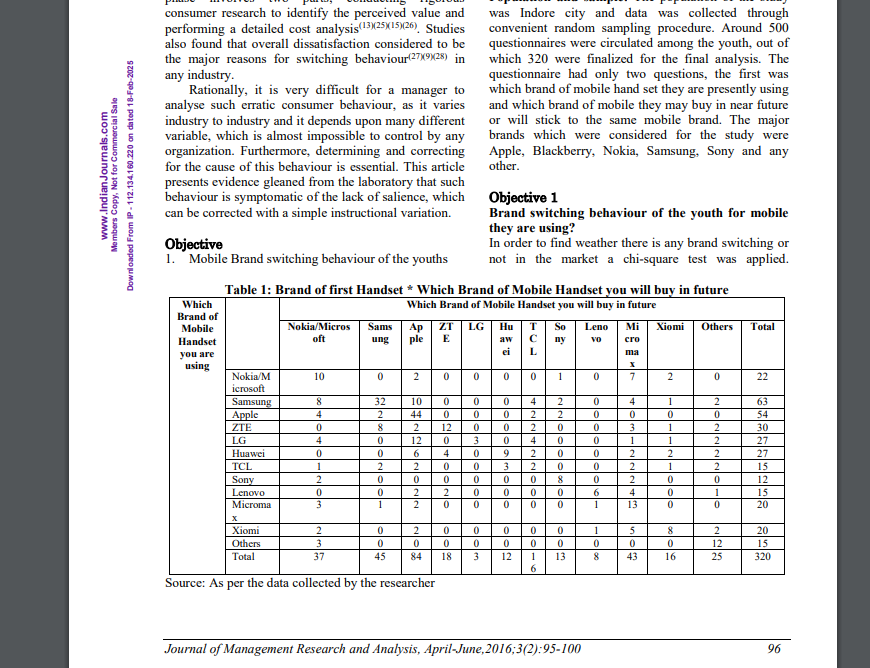
\includegraphics{ch6.1.png}

The above image is extracted from the paper ``Sharma, V., \& Sonwalkar,
J. (2016). Predicting the Switching Intention of Cell-Phone Brands:
Application of Markov Chain Models. Journal of Management Research and
Analysis, 3(2), 95-100.''

\subsection{Macroeconomic Modeling -- Analyzing business cycles and
economic growth using Markov
processes.}\label{macroeconomic-modeling-analyzing-business-cycles-and-economic-growth-using-markov-processes.}

\subsection{Income Distribution -- Modeling income mobility across
different economic
classes.}\label{income-distribution-modeling-income-mobility-across-different-economic-classes.}

\section{Finance}\label{finance}

\subsection{Stock Price Modeling -- The Markov property is fundamental
in models like the Black-Scholes
model.}\label{stock-price-modeling-the-markov-property-is-fundamental-in-models-like-the-black-scholes-model.}

\subsection{Credit Ratings -- Credit rating transitions of companies are
often modeled using Markov
chains.}\label{credit-ratings-credit-rating-transitions-of-companies-are-often-modeled-using-markov-chains.}

\subsection{Risk Management -- Estimating probabilities of financial
crises based on economic
indicators.}\label{risk-management-estimating-probabilities-of-financial-crises-based-on-economic-indicators.}

\section{Insurance}\label{insurance}

\subsection{Actuarial Science -- Predicting claim occurrences and
policyholder
behavior.}\label{actuarial-science-predicting-claim-occurrences-and-policyholder-behavior.}

\subsection{Risk Analysis -- Assessing life insurance risks with
Markovian mortality
models.}\label{risk-analysis-assessing-life-insurance-risks-with-markovian-mortality-models.}

\subsection{Policyholder Behavior -- Modeling lapse rates and claims
under different
conditions.}\label{policyholder-behavior-modeling-lapse-rates-and-claims-under-different-conditions.}

\bookmarksetup{startatroot}

\chapter{Summary}\label{summary}

In summary, this book has no content whatsoever.

\bookmarksetup{startatroot}

\chapter*{References}\label{references}
\addcontentsline{toc}{chapter}{References}

\markboth{References}{References}

\phantomsection\label{refs}
\begin{CSLReferences}{0}{1}
\end{CSLReferences}




\end{document}
